\documentclass[11pt,a4paper]{article}

%% ─── PACKAGES ────────────────────────────────────────────────────────────────
\usepackage[T1]{fontenc}
\usepackage[utf8]{inputenc}
\usepackage[a4paper, top=18mm, bottom=18mm, left=18mm, right=18mm]{geometry}
\usepackage[table]{xcolor}
\usepackage{amsmath}
\usepackage{amssymb}
\usepackage{microtype}
\usepackage{lmodern}
\usepackage{booktabs}
\usepackage{tabularx}
\usepackage{colortbl}
\usepackage{array}
\usepackage{multirow}
\usepackage{graphicx}
\usepackage{tikz}
\usepackage[most]{tcolorbox}
\usepackage{fontawesome5}
\usepackage{enumitem}
\usepackage{parskip}
\usepackage{setspace}
\usepackage{fancyhdr}
\usepackage{lastpage}
\usepackage{mdframed}
\usepackage{ifthen}
\usepackage{calc}
\usepackage{soul}

\usetikzlibrary{positioning, calc, shapes.geometric, backgrounds, patterns, decorations.pathmorphing}

%% ─── COLOUR PALETTE ──────────────────────────────────────────────────────────
\definecolor{RadBlue}{HTML}{1A3F6F}
\definecolor{RadTeal}{HTML}{2A8C8C}
\definecolor{RadSlate}{HTML}{4A5568}
\definecolor{RadLight}{HTML}{EBF4F7}
\definecolor{RadAccent}{HTML}{E8A020}
\definecolor{RadRule}{HTML}{CBD5E0}
\definecolor{RadBg}{HTML}{F7FAFC}
\definecolor{RadWhite}{HTML}{FFFFFF}
\definecolor{RadRed}{HTML}{C0392B}
\definecolor{RadGreen}{HTML}{27AE60}
\definecolor{RadAmber}{HTML}{E67E22}
\definecolor{RadLightBlue}{HTML}{DBEAFE}
\definecolor{RadHeaderBg}{HTML}{0F2A4A}

%% ─── TYPOGRAPHY ──────────────────────────────────────────────────────────────
\usepackage{lmodern}
\renewcommand{\familydefault}{\sfdefault}

%% ─── PAGE STYLE ──────────────────────────────────────────────────────────────
\pagestyle{fancy}
\fancyhf{}
\renewcommand{\headrulewidth}{0pt}
\renewcommand{\footrulewidth}{0pt}

\fancyfoot[L]{%
  \color{RadSlate}\footnotesize
  \textbf{Meridian Imaging Centre} \textbar{} Confidential Medical Record%
}
\fancyfoot[R]{%
  \color{RadSlate}\footnotesize
  Page \thepage\ of \pageref{LastPage}%
}
\fancyfoot[C]{%
  \color{RadRule}\footnotesize
  \rule{0pt}{8pt}%
}

%% ─── TCOLORBOX STYLES ────────────────────────────────────────────────────────
\tcbuselibrary{skins, breakable, fitting}

\tcbset{
  radbox/.style={
    enhanced,
    colback=RadWhite,
    colframe=RadBlue,
    arc=4pt,
    boxrule=1pt,
    left=8pt, right=8pt, top=6pt, bottom=6pt,
    fonttitle=\bfseries\color{RadWhite}\small,
    coltitle=RadWhite,
    attach boxed title to top left={yshift=-3mm, xshift=6mm},
    boxed title style={
      colback=RadBlue, colframe=RadBlue, arc=3pt, boxrule=0pt,
      left=4pt, right=4pt, top=2pt, bottom=2pt,
    },
  },
  tealbox/.style={
    enhanced,
    colback=RadLight,
    colframe=RadTeal,
    arc=4pt,
    boxrule=1pt,
    left=8pt, right=8pt, top=6pt, bottom=6pt,
    fonttitle=\bfseries\color{RadWhite}\small,
    coltitle=RadWhite,
    attach boxed title to top left={yshift=-3mm, xshift=6mm},
    boxed title style={
      colback=RadTeal, colframe=RadTeal, arc=3pt, boxrule=0pt,
      left=4pt, right=4pt, top=2pt, bottom=2pt,
    },
  },
  alertbox/.style={
    enhanced,
    colback=RadLightBlue,
    colframe=RadBlue,
    arc=4pt,
    boxrule=0.5pt,
    left=8pt, right=8pt, top=5pt, bottom=5pt,
  },
  slatebox/.style={
    enhanced,
    colback=RadBg,
    colframe=RadRule,
    arc=3pt,
    boxrule=0.6pt,
    left=7pt, right=7pt, top=5pt, bottom=5pt,
  },
}

%% ─── CUSTOM COMMANDS ─────────────────────────────────────────────────────────
\newcommand{\sectionrule}{%
  \vspace{2pt}%
  {\color{RadTeal}\rule{\linewidth}{1.5pt}}%
  \vspace{4pt}%
}

\newcommand{\subsectionrule}{%
  \vspace{1pt}%
  {\color{RadRule}\rule{\linewidth}{0.5pt}}%
  \vspace{3pt}%
}

\newcommand{\radfinding}[2]{%
  \noindent
  \begin{tcolorbox}[slatebox, left=7pt, right=7pt, top=4pt, bottom=4pt]
    \textbf{\color{RadBlue}#1}\hfill{\color{RadSlate}\small #2}
  \end{tcolorbox}%
  \vspace{2pt}%
}

\newcommand{\inforow}[2]{%
  \noindent
  {\color{RadSlate}\small\textbf{#1}}\hspace{4pt}{\color{black}\small #2}%
}

\newcommand{\findingbullet}[1]{%
  \item \small #1%
}

\newcommand{\imgbox}[3]{%
  \begin{tcolorbox}[
    enhanced,
    colback=RadHeaderBg,
    colframe=RadBlue,
    arc=4pt, boxrule=1pt,
    left=0pt, right=0pt, top=0pt, bottom=0pt,
    width=\linewidth,
    halign=center, valign=center,
  ]
    \begin{tikzpicture}[baseline]
      \fill[RadHeaderBg] (0,0) rectangle (#2,#3);
      \node[anchor=center, text=white!30!RadHeaderBg, font=\tiny] at (#2/2, #3/2) {};
      #1
    \end{tikzpicture}
  \end{tcolorbox}%
}

%% ─── SEVERITY BADGES ────────────────────────────────────────────────────────
\newcommand{\badgecritical}{%
  
\begin{tikzpicture}[baseline=-2pt]
    \node[fill=RadRed, text=white, font=\bfseries\tiny, inner xsep=5pt, inner ysep=2pt, rounded corners=3pt] {CRITICAL};
  \end{tikzpicture}%
}
\newcommand{\badgemoderately}{%
  
\begin{tikzpicture}[baseline=-2pt]
    \node[fill=RadAmber, text=white, font=\bfseries\tiny, inner xsep=5pt, inner ysep=2pt, rounded corners=3pt] {MODERATE};
  \end{tikzpicture}%
}
\newcommand{\badgenormal}{%
  
\begin{tikzpicture}[baseline=-2pt]
    \node[fill=RadGreen, text=white, font=\bfseries\tiny, inner xsep=5pt, inner ysep=2pt, rounded corners=3pt] {NORMAL};
  \end{tikzpicture}%
}
\newcommand{\badgemild}{%
  
\begin{tikzpicture}[baseline=-2pt]
    \node[fill=RadTeal, text=white, font=\bfseries\tiny, inner xsep=5pt, inner ysep=2pt, rounded corners=3pt] {MILD};
  \end{tikzpicture}%
}

%% ─── DOCUMENT ────────────────────────────────────────────────────────────────
\begin{document}

%% ═══════════════════════════════════════════════════════════════════════════
%% HEADER BLOCK
%% ═══════════════════════════════════════════════════════════════════════════
\thispagestyle{fancy}

\begin{tikzpicture}[remember picture, overlay]
  \fill[RadHeaderBg] (current page.north west) rectangle ([yshift=-38mm]current page.north east);
  \fill[RadTeal] ([yshift=-38mm]current page.north west) rectangle ([yshift=-40mm]current page.north east);
\end{tikzpicture}

\vspace*{-10mm}

\noindent
\begin{minipage}[t]{0.62\linewidth}
  \vspace{4mm}
  {\color{white}\fontsize{22}{26}\selectfont\bfseries Diagnostic Imaging Report}\\[2mm]
  {\color{RadTeal}\fontsize{11}{14}\selectfont\bfseries Meridian Imaging Centre}\\[1mm]
  {\color{white!70!RadHeaderBg}\small
    12 Radcliffe Boulevard, Suite 4A \textbar{} Harlington Medical Park\\
    Tel: +1 (604) 882-4100 \textbar{} Fax: +1 (604) 882-4199\\
    www.meridian-imaging.ca \textbar{} info@meridian-imaging.ca%
  }
\end{minipage}%
\hfill
\begin{minipage}[t]{0.35\linewidth}
  \vspace{4mm}
  \begin{tcolorbox}[
    enhanced, colback=RadBlue!80!black, colframe=RadTeal,
    arc=4pt, boxrule=1pt,
    left=7pt, right=7pt, top=6pt, bottom=6pt,
  ]
    \color{white}
    \small
    \textbf{\faFile\hspace{4pt}Report ID:}\hfill \texttt{MIC-2024-09471}\\[2pt]
    \textbf{\faCalendar\hspace{4pt}Date:}\hfill 14 November 2024\\[2pt]
    \textbf{\faClock\hspace{4pt}Time:}\hfill 09:47 AM\\[2pt]
    \textbf{\faFlask\hspace{4pt}Modality:}\hfill CT Thorax/Abdomen\\[2pt]
    \textbf{\faStar\hspace{4pt}Priority:}\hfill \badgecritical{}
  \end{tcolorbox}
\end{minipage}

\vspace{16mm}

%% ═══════════════════════════════════════════════════════════════════════════
%% PATIENT DEMOGRAPHICS
%% ═══════════════════════════════════════════════════════════════════════════

\begin{tcolorbox}[radbox, title={\faUser\hspace{4pt}Patient Information}]
\vspace{4pt}
\begin{tabular}{@{}p{0.22\linewidth}p{0.27\linewidth}p{0.18\linewidth}p{0.25\linewidth}@{}}
  \small\color{RadSlate}\textbf{Full Name} &
  \small Margaret A. Holloway &
  \small\color{RadSlate}\textbf{Date of Birth} &
  \small 03 June 1967 (Age 57) \\[4pt]
  \small\color{RadSlate}\textbf{Patient ID} &
  \small \texttt{PAT-00192834} &
  \small\color{RadSlate}\textbf{Sex / Gender} &
  \small Female \\[4pt]
  \small\color{RadSlate}\textbf{MRN} &
  \small \texttt{MRN-7743-H} &
  \small\color{RadSlate}\textbf{Weight / Height} &
  \small 68 kg \textbar{} 164 cm \\[4pt]
  \small\color{RadSlate}\textbf{Referring Physician} &
  \small Dr. Thomas B. Crane, MD &
  \small\color{RadSlate}\textbf{Insurance} &
  \small Apex Health Plan \\[4pt]
  \small\color{RadSlate}\textbf{Ward / Location} &
  \small Outpatient -- Level 2 &
  \small\color{RadSlate}\textbf{Accession No.} &
  \small \texttt{ACC-2024-48173} \\
\end{tabular}
\vspace{4pt}
\end{tcolorbox}

\vspace{6pt}

%% ─── CLINICAL HISTORY ────────────────────────────────────────────────────────

\begin{tcolorbox}[tealbox, title={\faClipboardList\hspace{4pt}Clinical History \& Indication}]
\small
The patient presents with a 6-week history of progressive dyspnoea on exertion, intermittent pleuritic chest pain (right-sided), and a persistent dry cough unresponsive to empirical antibiotic therapy. Past medical history is notable for hypertension (treated with amlodipine 5 mg daily), a remote right knee arthroscopy (2009), and a family history of pulmonary malignancy (maternal uncle). No smoking history. The referring physician has requested CT thorax with contrast and CT upper abdomen to evaluate for pulmonary embolism, parenchymal pathology, and occult mediastinal lymphadenopathy.
\end{tcolorbox}

\vspace{6pt}

%% ─── TECHNIQUE ───────────────────────────────────────────────────────────────

\begin{tcolorbox}[slatebox, title=]
\noindent\textbf{\color{RadBlue}\faTools\hspace{4pt}Examination Technique}
\vspace{4pt}

\subsectionrule{}

\small\setlength{\tabcolsep}{4pt}
\begin{tabular}{@{}p{0.17\linewidth}p{0.30\linewidth}p{0.17\linewidth}p{0.30\linewidth}@{}}
  \color{RadSlate}\textbf{Scanner} & Synapse 64-Slice CT & \color{RadSlate}\textbf{kVp / mAs} & 120 kVp / 280 mAs \\[3pt]
  \color{RadSlate}\textbf{Protocol} & Contrast-Enhanced (CECT) & \color{RadSlate}\textbf{Slice Thickness} & 1.5 mm axial, MPR coronal/sagittal \\[3pt]
  \color{RadSlate}\textbf{Contrast Agent} & Omniscan IV 100 mL & \color{RadSlate}\textbf{Injection Rate} & 3.5 mL/s via right antecubital IV \\[3pt]
  \color{RadSlate}\textbf{Scout View} & PA chest + lateral & \color{RadSlate}\textbf{Radiation Dose} & CTDIvol 8.4 mGy; DLP 420 mGy$\cdot$cm \\[3pt]
  \color{RadSlate}\textbf{Breathing Phase} & Inspiration / expiration & \color{RadSlate}\textbf{Reconstruction} & Lung window + mediastinal window \\
\end{tabular}
\end{tcolorbox}

\vspace{8pt}

%% ═══════════════════════════════════════════════════════════════════════════
%% IMAGE PANEL (simulated with tikz)
%% ═══════════════════════════════════════════════════════════════════════════

\noindent\textbf{\color{RadBlue}\fontsize{11}{13}\selectfont\faImage\hspace{4pt}Key Image Panel}
\vspace{4pt}

\sectionrule{}

\vspace{2pt}

\noindent
\begin{minipage}[t]{0.325\linewidth}
  \begin{tcolorbox}[
    enhanced, colback=RadHeaderBg, colframe=RadBlue,
    arc=4pt, boxrule=1pt,
    left=0pt, right=0pt, top=0pt, bottom=0pt,
  ]
    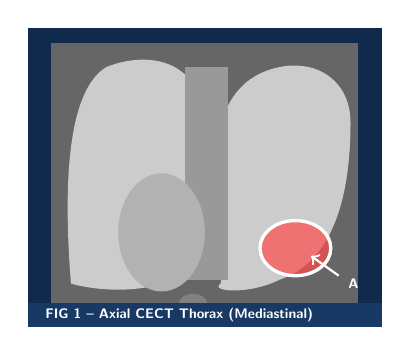
\begin{tikzpicture}
      \fill[RadHeaderBg] (0,0) rectangle (4.5,3.8);
      %% Simulated lung CT slice
      \fill[black!60] (0.3,0.2) rectangle (4.2,3.6);
      %% Left lung outline
      \fill[black!20] (0.55,0.55) .. controls (0.45,1.8) and (0.5,3.0) .. (1.0,3.3)
                      .. controls (1.5,3.5) and (2.1,3.4) .. (2.2,2.8)
                      .. controls (2.3,2.2) and (2.2,1.2) .. (2.0,0.7)
                      .. controls (1.6,0.4) and (0.9,0.45) .. (0.55,0.55);
      %% Right lung outline
      \fill[black!20] (2.45,0.55) .. controls (2.3,0.45) and (2.8,0.4) .. (3.2,0.6)
                      .. controls (3.8,0.8) and (4.1,1.5) .. (4.1,2.6)
                      .. controls (4.1,3.1) and (3.7,3.4) .. (3.2,3.3)
                      .. controls (2.7,3.2) and (2.4,2.8) .. (2.4,2.1)
                      .. controls (2.4,1.3) and (2.5,0.7) .. (2.45,0.55);
      %% Mediastinum
      \fill[black!40] (2.0,0.6) rectangle (2.55,3.3);
      %% Pulmonary lesion highlight (right lower lobe)
      \fill[white!30!red, opacity=0.7] (3.4,1.0) ellipse ({0.45} and {0.35});
      \draw[white, very thick] (3.4,1.0) ellipse ({0.45} and {0.35});
      %% Annotation arrow
      \draw[white, thick, ->] (3.95,0.65) -- (3.6,0.9);
      \node[white, font=\tiny\bfseries, anchor=west] at (3.95,0.55) {A};
      %% Vertebrae hint
      \fill[black!50] (2.1,0.3) ellipse ({0.18} and {0.12});
      %% Heart shadow
      \fill[black!30] (1.7,1.2) ellipse ({0.55} and {0.75});
      %% Label bar at bottom
      \fill[RadBlue!90!black] (0,0) rectangle (4.5,0.3);
      \node[white, font=\tiny\bfseries, anchor=west] at (0.1,0.15) {FIG 1 -- Axial CECT Thorax (Mediastinal)};
    \end{tikzpicture}
  \end{tcolorbox}
  \vspace{3pt}
  \begin{tcolorbox}[slatebox, left=5pt, right=5pt, top=3pt, bottom=3pt]
    \tiny\color{RadSlate}
    \textbf{Fig 1:} Right lower lobe lesion (arrow A). Size: 28 $\times$ 22 mm. Irregular margin, mild pleural contact. Level: T8.
  \end{tcolorbox}
\end{minipage}%
\hfill
\begin{minipage}[t]{0.325\linewidth}
  \begin{tcolorbox}[
    enhanced, colback=RadHeaderBg, colframe=RadTeal,
    arc=4pt, boxrule=1pt,
    left=0pt, right=0pt, top=0pt, bottom=0pt,
  ]
    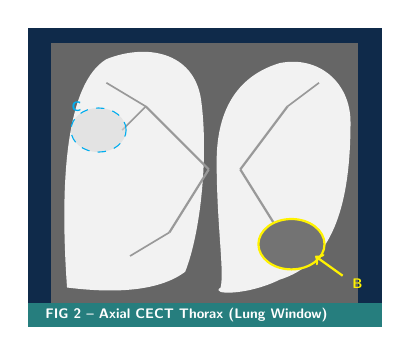
\begin{tikzpicture}
      \fill[RadHeaderBg] (0,0) rectangle (4.5,3.8);
      \fill[black!60] (0.3,0.2) rectangle (4.2,3.6);
      %% Lung window -- high contrast
      \fill[black!5] (0.5,0.5) .. controls (0.4,1.9) and (0.5,3.1) .. (1.0,3.4)
                     .. controls (1.5,3.6) and (2.1,3.5) .. (2.2,2.9)
                     .. controls (2.3,2.2) and (2.2,1.2) .. (2.0,0.7)
                     .. controls (1.6,0.4) and (0.9,0.45) .. (0.5,0.5);
      \fill[black!5] (2.45,0.5) .. controls (2.3,0.4) and (2.8,0.4) .. (3.2,0.6)
                     .. controls (3.85,0.8) and (4.1,1.5) .. (4.1,2.6)
                     .. controls (4.1,3.1) and (3.7,3.45) .. (3.2,3.35)
                     .. controls (2.7,3.2) and (2.4,2.8) .. (2.4,2.1)
                     .. controls (2.4,1.3) and (2.5,0.7) .. (2.45,0.5);
      %% Pulmonary vessels (branching)
      \draw[black!40, line width=0.8pt] (2.3,2.0) -- (1.5,2.8);
      \draw[black!40, line width=0.6pt] (1.5,2.8) -- (1.0,3.1);
      \draw[black!40, line width=0.6pt] (1.5,2.8) -- (1.2,2.5);
      \draw[black!40, line width=0.8pt] (2.3,2.0) -- (1.8,1.2);
      \draw[black!40, line width=0.6pt] (1.8,1.2) -- (1.3,0.9);
      \draw[black!40, line width=0.8pt] (2.7,2.0) -- (3.3,2.8);
      \draw[black!40, line width=0.6pt] (3.3,2.8) -- (3.7,3.1);
      \draw[black!40, line width=0.8pt] (2.7,2.0) -- (3.2,1.2);
      \draw[black!40, line width=0.6pt] (3.2,1.2) -- (3.7,0.9);
      %% Lesion in lung window
      \fill[black!55] (3.35,1.05) ellipse ({0.42} and {0.32});
      \draw[yellow, thick] (3.35,1.05) ellipse ({0.42} and {0.32});
      %% Annotation
      \draw[yellow, thick, ->] (4.0,0.65) -- (3.65,0.9);
      \node[yellow, font=\tiny\bfseries, anchor=west] at (4.0,0.55) {B};
      %% Ground glass opacity (left upper)
      \fill[black!15, opacity=0.6] (0.9,2.5) ellipse ({0.35} and {0.28});
      \draw[cyan, dashed, thin] (0.9,2.5) ellipse ({0.35} and {0.28});
      \node[cyan, font=\tiny\bfseries] at (0.62,2.8) {C};
      %% Label
      \fill[RadTeal!90!black] (0,0) rectangle (4.5,0.3);
      \node[white, font=\tiny\bfseries, anchor=west] at (0.1,0.15) {FIG 2 -- Axial CECT Thorax (Lung Window)};
    \end{tikzpicture}
  \end{tcolorbox}
  \vspace{3pt}
  \begin{tcolorbox}[slatebox, left=5pt, right=5pt, top=3pt, bottom=3pt]
    \tiny\color{RadSlate}
    \textbf{Fig 2:} Same lesion (arrow B, lung window). Ground glass haze left upper lobe (arrow C), no central necrosis.
  \end{tcolorbox}
\end{minipage}%
\hfill
\begin{minipage}[t]{0.325\linewidth}
  \begin{tcolorbox}[
    enhanced, colback=RadHeaderBg, colframe=RadSlate,
    arc=4pt, boxrule=1pt,
    left=0pt, right=0pt, top=0pt, bottom=0pt,
  ]
    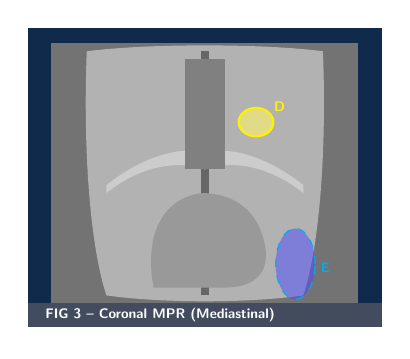
\begin{tikzpicture}
      \fill[RadHeaderBg] (0,0) rectangle (4.5,3.8);
      \fill[black!55] (0.3,0.2) rectangle (4.2,3.6);
      %% Coronal view -- body silhouette
      \fill[black!30] (1.0,0.4) .. controls (0.8,1.0) and (0.7,2.2) .. (0.75,3.5)
                      .. controls (1.5,3.6) and (3.0,3.6) .. (3.75,3.5)
                      .. controls (3.8,2.2) and (3.7,1.0) .. (3.5,0.4)
                      .. controls (2.8,0.3) and (1.7,0.3) .. (1.0,0.4);
      %% Spine
      \draw[black!60, line width=3pt] (2.25,0.4) -- (2.25,3.5);
      %% Diaphragm domes
      \fill[black!20] (1.0,1.8) .. controls (1.5,2.2) and (2.0,2.3) .. (2.25,2.2)
                      .. controls (2.5,2.3) and (3.0,2.2) .. (3.5,1.8)
                      -- (3.5,1.7) .. controls (3.0,2.1) and (2.5,2.1) .. (2.25,2.0)
                      .. controls (2.0,2.1) and (1.5,2.1) .. (1.0,1.7) -- cycle;
      %% Abdominal organs (liver shadow)
      \fill[black!40] (1.6,0.5) .. controls (1.5,1.0) and (1.6,1.6) .. (2.2,1.7)
                      .. controls (2.6,1.7) and (2.9,1.5) .. (3.0,1.1)
                      .. controls (3.1,0.7) and (2.9,0.5) .. (2.5,0.5) -- cycle;
      %% Mediastinum
      \fill[black!50] (2.0,2.0) rectangle (2.5,3.4);
      %% Hilar lymph node (right)
      \fill[white!40!yellow, opacity=0.6] (2.9,2.6) ellipse ({0.22} and {0.18});
      \draw[yellow, thick] (2.9,2.6) ellipse ({0.22} and {0.18});
      \node[yellow, font=\tiny\bfseries] at (3.2,2.8) {D};
      %% Right pleural effusion
      \fill[white!30!blue, opacity=0.5] (3.4,0.8) ellipse ({0.25} and {0.45});
      \draw[cyan, dashed] (3.4,0.8) ellipse ({0.25} and {0.45});
      \node[cyan, font=\tiny\bfseries] at (3.78,0.75) {E};
      %% Label
      \fill[RadSlate!90!black] (0,0) rectangle (4.5,0.3);
      \node[white, font=\tiny\bfseries, anchor=west] at (0.1,0.15) {FIG 3 -- Coronal MPR (Mediastinal)};
    \end{tikzpicture}
  \end{tcolorbox}
  \vspace{3pt}
  \begin{tcolorbox}[slatebox, left=5pt, right=5pt, top=3pt, bottom=3pt]
    \tiny\color{RadSlate}
    \textbf{Fig 3:} Right hilar lymph node (D, 14 mm). Small right pleural effusion (E). No mediastinal shift.
  \end{tcolorbox}
\end{minipage}

\vspace{10pt}

%% ═══════════════════════════════════════════════════════════════════════════
%% FINDINGS
%% ═══════════════════════════════════════════════════════════════════════════

\noindent\textbf{\color{RadBlue}\fontsize{11}{13}\selectfont\faMicroscope\hspace{4pt}Radiological Findings}
\vspace{4pt}

\sectionrule{}

\vspace{4pt}

%% Chest
\begin{tcolorbox}[radbox, title={\faLungs\hspace{4pt}Thorax -- Parenchyma \& Airways}]
\vspace{4pt}
\begin{itemize}[leftmargin=14pt, itemsep=3pt, parsep=0pt]
  \findingbullet{\textbf{Right Lower Lobe Mass (Segment 6):} A well-defined spiculate soft-tissue density nodule measuring \textbf{28 $\times$ 22 $\times$ 20 mm} is identified in the posterior right lower lobe (Figs 1 and 2, annotation A/B). The lesion demonstrates heterogeneous enhancement (HU pre: 28; HU post: 67). Margins are lobulated with pleural tethering. No cavitation or calcification.}
  \findingbullet{\textbf{Ground Glass Opacity -- Left Upper Lobe:} A \textbf{12 $\times$ 9 mm} area of ground glass attenuation in the anterior segment of the left upper lobe (Fig 2, annotation C). No consolidation or air-bronchogram. Stable pattern; unchanged from prior CT (16 June 2024). Likely represents sub-acute inflammatory change.}
  \findingbullet{\textbf{Airways:} Trachea midline. Main bronchi patent. No endobronchial lesion. Mild wall thickening of the right lower lobe bronchus, consistent with peribronchial cuffing. No mucous plugging.}
  \findingbullet{\textbf{Pleura:} Small right-sided pleural effusion estimated at 60--80 mL (Fig 3, annotation E). No left effusion. No pneumothorax. No empyema.}
\end{itemize}
\vspace{4pt}
\end{tcolorbox}

\vspace{6pt}

%% Two minipages for next two finding boxes
\noindent
\begin{minipage}[t]{0.49\linewidth}
\begin{tcolorbox}[tealbox, title={\faHeart\hspace{4pt}Mediastinum \& Cardiovascular}]
\vspace{4pt}
\begin{itemize}[leftmargin=12pt, itemsep=3pt, parsep=0pt]
  \findingbullet{\textbf{Heart:} Mildly enlarged (CTR $\approx$0.53). No pericardial effusion. Coronary artery calcification: mild LAD deposits (Agatston $\approx$ 42).}
  \findingbullet{\textbf{Aorta:} Normal calibre ascending (30 mm) and descending (22 mm) aorta. No aneurysm or dissection.}
  \findingbullet{\textbf{Pulmonary Arteries:} No filling defect in central or lobar pulmonary arteries to indicate PE. Subsegmental vessels not fully evaluated.}
  \findingbullet{\textbf{Lymph Nodes:} Right hilar node 14 mm short axis (Fig 3, arrow D) -- borderline enlarged. Right paratracheal station 4R node 9 mm. No mediastinal bulk.}
\end{itemize}
\vspace{4pt}
\end{tcolorbox}
\end{minipage}%
\hfill
\par
\begin{minipage}[t]{0.49\linewidth}
\begin{tcolorbox}[tealbox, title={\faStethoscope\hspace{4pt}Upper Abdomen (Limited)}]
\vspace{4pt}
\begin{itemize}[leftmargin=12pt, itemsep=3pt, parsep=0pt]
  \findingbullet{\textbf{Liver:} Homogeneous parenchyma. No focal lesion. Normal hepatic veins. Mild fatty change (HU 42).}
  \findingbullet{\textbf{Gallbladder \& Biliary:} Gallbladder present; two small non-obstructing gallstones (max 8 mm). Common bile duct 5 mm -- within normal limits.}
  \findingbullet{\textbf{Spleen / Pancreas / Adrenals:} Spleen 11 cm, homogeneous. Pancreas unremarkable. Adrenal glands symmetric, no adenoma.}
  \findingbullet{\textbf{Kidneys:} Both kidneys normal size and enhancement. A 6 mm simple cortical cyst right kidney (Bosniak I).}
\end{itemize}
\vspace{4pt}
\end{tcolorbox}
\end{minipage}

\vspace{8pt}

%% ─── MEASUREMENTS TABLE ──────────────────────────────────────────────────────

\begin{tcolorbox}[slatebox]
\noindent\textbf{\color{RadBlue}\faRuler\hspace{4pt}Lesion Measurement Summary}
\vspace{5pt}

\subsectionrule{}

\small
\setlength{\tabcolsep}{5pt}
\renewcommand{\arraystretch}{1.35}
\begin{tabular}{@{}lllllll@{}}
  \toprule
  \rowcolor{RadBlue}
  \color{white}\textbf{Lesion} &
  \color{white}\textbf{Location} &
  \color{white}\textbf{Size (mm)} &
  \color{white}\textbf{HU Pre} &
  \color{white}\textbf{HU Post} &
  \color{white}\textbf{Enhancement} &
  \color{white}\textbf{Status} \\
  \midrule{}
  RLL Spiculate Mass & Post Seg 6, RLL & $28\times22\times20$ & 28 & 67 & +39 HU & \badgecritical{} \\
  \rowcolor{RadBg}
  LUL Ground Glass & Ant Seg, LUL & $12\times9$ & --10 & --8 & Minimal & \badgemild{} \\
  R Hilar Lymph Node & Station 10R & $14\times11$ & 32 & 58 & +26 HU & \badgemoderately{} \\
  \rowcolor{RadBg}
  R Pleural Effusion & Right Pleural Space & $\sim$60--80 mL & -- & -- & N/A & \badgemoderately{} \\
  LAD Calcification & Proximal LAD & Agatston 42 & -- & -- & N/A & \badgemild{} \\
  \rowcolor{RadBg}
  Right Renal Cyst & Upper Pole, RK & 6 & 5 & 6 & None & \badgenormal{} \\
  \bottomrule
\end{tabular}
\end{tcolorbox}

\vspace{8pt}

%% ═══════════════════════════════════════════════════════════════════════════
%% IMPRESSION & RECOMMENDATIONS
%% ═══════════════════════════════════════════════════════════════════════════

\begin{tcolorbox}[
  enhanced,
  colback=RadHeaderBg,
  colframe=RadTeal,
  arc=5pt,
  boxrule=1.5pt,
  left=10pt, right=10pt, top=8pt, bottom=8pt,
  title={\faExclamationTriangle\hspace{4pt}Radiological Impression},
  fonttitle=\bfseries\color{RadWhite}\normalsize,
  coltitle=RadWhite,
  attach boxed title to top left={yshift=-3mm, xshift=8mm},
  boxed title style={
    colback=RadTeal, colframe=RadTeal, arc=3pt, boxrule=0pt,
    left=5pt, right=5pt, top=2pt, bottom=2pt,
  },
]
\vspace{4pt}
\color{white}
\begin{enumerate}[leftmargin=18pt, label=\textbf{\arabic*.}, itemsep=4pt, parsep=0pt]
  \item \textbf{Spiculate right lower lobe mass (28 mm):} The morphological characteristics --- lobulated margin, pleural tethering, and moderate post-contrast enhancement --- are highly suspicious for primary lung malignancy (clinical T1c N1 staging pending PET-CT). \textbf{Urgent multidisciplinary tumour board discussion is recommended.}
  \item \textbf{Borderline right hilar lymphadenopathy (14 mm):} In the clinical context, this raises concern for regional nodal involvement. PET-CT and/or endobronchial ultrasound (EBUS) guided biopsy advised.
  \item \textbf{Small right pleural effusion:} Likely reactive; may warrant thoracocentesis for cytological analysis if increasing on follow-up.
  \item \textbf{Left upper lobe ground glass opacity:} Indeterminate but stable on comparison. Repeat HRCT in 3 months if current lesion is confirmed malignant.
  \item \textbf{Incidental findings:} Mild left ventricular enlargement (clinical correlation); gallstones (conservative management); right renal Bosniak I cyst (no follow-up needed).
\end{enumerate}
\vspace{4pt}
\end{tcolorbox}

\vspace{8pt}

%% ─── RECOMMENDATIONS ────────────────────────────────────────────────────────

\begin{tcolorbox}[radbox, title={\faList\hspace{4pt}Recommended Next Steps}]
\vspace{4pt}
\small
\begin{tabular}{@{}p{0.04\linewidth}p{0.88\linewidth}@{}}
  \textbf{1.} & \textbf{PET-CT whole body} within 5 working days for accurate staging of the RLL mass. \\[4pt]
  \textbf{2.} & \textbf{Bronchoscopy $\pm$ EBUS-TBNA} to obtain histopathological diagnosis and nodal sampling of station 10R/4R. \\[4pt]
  \textbf{3.} & \textbf{Pulmonary function tests (PFTs)} prior to any surgical consideration. \\[4pt]
  \textbf{4.} & \textbf{Cardiology referral} re: coronary artery calcification and mild cardiomegaly. \\[4pt]
  \textbf{5.} & \textbf{Multidisciplinary Tumour Board (MDT)} review -- please submit imaging and pathology results to the Thoracic Oncology MDT (Meridian Apex Oncology Network). \\[4pt]
  \textbf{6.} & Comparison with any outside imaging obtainable -- referring physician to arrange transfer of prior studies. \\
\end{tabular}
\vspace{4pt}
\end{tcolorbox}

\vspace{8pt}

%% ─── COMPARISON / PRIOR STUDIES ──────────────────────────────────────────────

\begin{tcolorbox}[slatebox]
\noindent\textbf{\color{RadBlue}\faHistory\hspace{4pt}Prior Study Comparison}
\vspace{4pt}

\subsectionrule{}

\small
\begin{tabular}{@{}llll@{}}
  \toprule
  \textbf{Study Date} & \textbf{Modality} & \textbf{Institution} & \textbf{Relevant Finding} \\
  \midrule{}
  16 June 2024 & CT Thorax (non-contrast) & Apex Diagnostic Labs & LUL GGO 11 mm (stable); no RLL mass reported \\
  \rowcolor{RadBg}
  03 Feb 2024 & Chest X-Ray PA & Nexa Community Clinic & RLL opacity, attributed to infection; no follow-up \\
  09 Nov 2022 & CT Thorax (non-contrast) & Meridian Imaging Centre & No parenchymal mass; normal hilar silhouette \\
  \bottomrule
\end{tabular}

\vspace{6pt}
\noindent{\color{RadAmber}\faExclamationTriangle}\hspace{4pt}\small\textbf{Note:} The RLL mass appears to represent an interval development between June 2024 and November 2024, underscoring the need for urgent histological evaluation.
\end{tcolorbox}

\vspace{10pt}

%% ═══════════════════════════════════════════════════════════════════════════
%% SIGNATURE / ATTESTATION BLOCK
%% ═══════════════════════════════════════════════════════════════════════════

\begin{tcolorbox}[slatebox]
\noindent\textbf{\color{RadBlue}\faPen\hspace{4pt}Reporting Radiologist}
\vspace{5pt}

\subsectionrule{}

\vspace{2pt}
\noindent
\begin{minipage}[t]{0.55\linewidth}
  \small
  \textbf{Name:} Dr. Rachel S. Thornton, FRCR, FCAR\\[2pt]
  \textbf{Subspecialty:} Cardiothoracic \& Oncologic Radiology\\[2pt]
  \textbf{Licence No.:} CPSBC-74291-R\\[2pt]
  \textbf{Institution:} Meridian Imaging Centre, Harlington\\[2pt]
  \textbf{Report Prepared:} 14 November 2024, 11:32 AM\\[2pt]
  \textbf{Electronically Verified:} 14 November 2024, 13:05 PM\\[4pt]
  \begin{tcolorbox}[
    enhanced, colback=RadLight, colframe=RadTeal, arc=3pt, boxrule=0.5pt,
    left=6pt, right=6pt, top=4pt, bottom=4pt,
  ]
    \tiny\color{RadSlate}
    \textit{This report was generated and electronically signed by the above-named radiologist. Results have been communicated to the referring physician Dr. T. B. Crane via secure EMR portal. This document constitutes a confidential medical record.}
  \end{tcolorbox}
\end{minipage}%
\hfill
\begin{minipage}[t]{0.40\linewidth}
  \vspace{2mm}
  
\begin{tikzpicture}
    \draw[RadRule, thick] (0,0) rectangle (5.2,1.4);
    \fill[RadBg] (0,0) rectangle (5.2,1.4);
    \node[font=\large\bfseries\color{RadBlue}, anchor=center] at (2.6,0.9) {\textit{Rachel S. Thornton}};
    \draw[RadSlate, thick] (0.3,0.45) -- (4.9,0.45);
    \node[font=\tiny\color{RadSlate}, anchor=center] at (2.6,0.2) {Signature / Electronic Authentication};
    %% Seal circle
    \draw[RadTeal, thick] (4.3,1.1) circle (0.25);
    \node[RadTeal, font=\tiny\bfseries, anchor=center] at (4.3,1.1) {\faStar};
  \end{tikzpicture}

  \vspace{3mm}
  \noindent
  \begin{tcolorbox}[
    enhanced, colback=RadLightBlue, colframe=RadBlue, arc=3pt, boxrule=0.5pt,
    left=5pt, right=5pt, top=4pt, bottom=4pt,
  ]
    \tiny\color{RadBlue}
    \textbf{QA Reviewed By:} Dr. Alan Park, MD, FRCR\\
    \textbf{QA Date:} 14 Nov 2024, 13:05 PM\\
    \textbf{Peer Review Score:} 4 / 4 (Concordant)
  \end{tcolorbox}
\end{minipage}
\end{tcolorbox}

\vspace{8pt}

%% ─── FOOTER DISCLAIMER ──────────────────────────────────────────────────────

\begin{tcolorbox}[
  enhanced,
  colback=RadBg,
  colframe=RadRule,
  arc=3pt, boxrule=0.5pt,
  left=8pt, right=8pt, top=4pt, bottom=4pt,
]
\tiny\color{RadSlate}
\textbf{CONFIDENTIALITY NOTICE:} This radiology report is intended solely for the named referring clinician and the treating medical team responsible for the care of the identified patient. It may contain protected health information (PHI) subject to applicable privacy regulations. Any unauthorised review, use, disclosure, or distribution is strictly prohibited. If you have received this document in error, please contact Meridian Imaging Centre immediately at +1 (604) 882-4100 and destroy all copies. \textbf{Meridian Imaging Centre is not liable for clinical decisions made without direct consultation with the reporting radiologist.}
\end{tcolorbox}

\newpage

%% ═══════════════════════════════════════════════════════════════════════════
%% PAGE 2: ADDENDUM / STRUCTURED REPORTING METRICS
%% ═══════════════════════════════════════════════════════════════════════════

\noindent\textbf{\color{RadBlue}\fontsize{13}{16}\selectfont Structured Reporting Addendum}
\vspace{3pt}

\sectionrule{}

\vspace{4pt}

%% Lung-RADS and scoring
\begin{tcolorbox}[radbox, title={\faChartBar\hspace{4pt}Lung-RADS 2022 Assessment Category}]
\vspace{4pt}
\noindent
\begin{minipage}[t]{0.55\linewidth}
\small
\begin{tabular}{@{}p{0.42\linewidth}p{0.52\linewidth}@{}}
  \textbf{Category:} & \textbf{4X -- Suspicious (Category 4)} \\[4pt]
  \textbf{Modifier:} & X (additional imaging/clinical info) \\[4pt]
  \textbf{Malignancy Risk:} & $>$15\% \\[4pt]
  \textbf{Management:} & Diagnostic CT, PET-CT, tissue sampling \\[4pt]
  \textbf{Prior Category:} & 2 (June 2024, non-contrast CT) \\[4pt]
  \textbf{Change:} & Upgrade from Cat 2 $\to$ Cat 4X \\
\end{tabular}
\end{minipage}%
\hfill
\begin{minipage}[t]{0.40\linewidth}
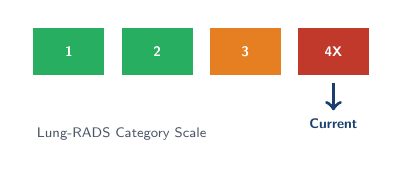
\begin{tikzpicture}
  \foreach \c/\lbl/\col in {
    1/1/RadGreen,
    2/2/RadGreen,
    3/3/RadAmber,
    4/4X/RadRed}{
    \pgfmathsetmacro{\xpos}{(\c-1)*1.12}
    \fill[\col] (\xpos,0) rectangle (\xpos+0.9,0.6);
    \node[white, font=\tiny\bfseries] at (\xpos+0.45,0.3) {\lbl};
  }
  \draw[RadBlue, very thick, ->] (3*1.12+0.45,-0.1) -- (3*1.12+0.45,-0.45);
  \node[RadBlue, font=\tiny\bfseries] at (3*1.12+0.45,-0.62) {Current};
  \node[RadSlate, font=\tiny] at (2*0.56,-0.75) {Lung-RADS Category Scale};
\end{tikzpicture}
\end{minipage}
\vspace{4pt}
\end{tcolorbox}

\vspace{6pt}

%% TNM provisional staging
\begin{tcolorbox}[tealbox, title={\faDna\hspace{4pt}Provisional Radiological TNM Staging (8th Ed.)}]
\vspace{4pt}
\small
\begin{tabular}{@{}p{0.12\linewidth}p{0.35\linewidth}p{0.12\linewidth}p{0.35\linewidth}@{}}
  \textbf{T Stage:} & T2a (tumour $>$2 cm, $\leq$3 cm) & \textbf{N Stage:} & N1 (ipsilateral hilar node) \\[4pt]
  \textbf{M Stage:} & Mx (distant metastasis not assessed) & \textbf{Group:} & IIB (T2a N1 Mx) -- provisional \\[4pt]
  \textbf{Histology:} & Pending biopsy & \textbf{AJCC Group:} & IIB \\
\end{tabular}
\vspace{4pt}

\noindent{\color{RadAmber}\textbf{\faExclamationCircle\hspace{3pt}Important:}} Radiological staging is provisional. Final staging requires histopathological and PET-CT data. Management decisions must not be based on imaging alone.
\vspace{4pt}
\end{tcolorbox}

\vspace{6pt}

%% Structured data / protocol compliance
\noindent
\begin{minipage}[t]{0.48\linewidth}
\begin{tcolorbox}[radbox, title={\faLock\hspace{4pt}Radiation Dose Record}]
\vspace{4pt}
\small
\begin{tabular}{@{}p{0.52\linewidth}p{0.42\linewidth}@{}}
  \textbf{CTDIvol:} & 8.4 mGy \\[3pt]
  \textbf{DLP:} & 420 mGy$\cdot$cm \\[3pt]
  \textbf{SSDE:} & 9.1 mGy \\[3pt]
  \textbf{Scan Length:} & 490 mm \\[3pt]
  \textbf{Diagnostic Ref. Level:} & Below national DRL \\[3pt]
  \textbf{As Low As Reasonably:} & Achieved (ALARA) \\
\end{tabular}
\vspace{4pt}
\end{tcolorbox}
\end{minipage}%
\hfill
\par
\begin{minipage}[t]{0.48\linewidth}
\begin{tcolorbox}[radbox, title={\faVial\hspace{4pt}Contrast Administration Record}]
\vspace{4pt}
\small
\begin{tabular}{@{}p{0.52\linewidth}p{0.42\linewidth}@{}}
  \textbf{Agent:} & Iodixanol (Omniscan) \\[3pt]
  \textbf{Concentration:} & 320 mgI/mL \\[3pt]
  \textbf{Volume:} & 100 mL IV \\[3pt]
  \textbf{Rate:} & 3.5 mL/s \\[3pt]
  \textbf{eGFR (pre-scan):} & 74 mL/min/1.73m$^{2}$ \\[3pt]
  \textbf{Adverse Reaction:} & None observed \\
\end{tabular}
\vspace{4pt}
\end{tcolorbox}
\end{minipage}

\vspace{8pt}

%% Differential diagnosis table
\begin{tcolorbox}[slatebox]
\noindent\textbf{\color{RadBlue}\faBalanceScale\hspace{4pt}Differential Diagnosis}
\vspace{5pt}

\subsectionrule{}

\small
\renewcommand{\arraystretch}{1.35}
\begin{tabular}{@{}p{0.03\linewidth}p{0.27\linewidth}p{0.14\linewidth}p{0.49\linewidth}@{}}
  \toprule
  \textbf{\#} & \textbf{Diagnosis} & \textbf{Likelihood} & \textbf{Supporting / Against Features} \\
  \midrule{}
  1 & Primary lung adenocarcinoma & Very High & Spiculate margins, enhancement pattern, RLL location, hilar node; age/sex profile \\
  \rowcolor{RadBg}
  2 & Squamous cell carcinoma & Moderate & Central-ish hilar node; lacks cavitation and squamous cell classic features \\
  3 & Pulmonary carcinoid & Low & Enhancement higher than expected; location atypical \\
  \rowcolor{RadBg}
  4 & Metastatic deposit & Low & No known primary; single lesion; no prior malignancy history \\
  5 & Organising pneumonia & Very Low & No prior antibiotic response; spiculate morphology atypical \\
  \bottomrule
\end{tabular}
\end{tcolorbox}

\vspace{8pt}

%% Quality metrics
\begin{tcolorbox}[
  enhanced,
  colback=RadLight,
  colframe=RadTeal,
  arc=4pt, boxrule=1pt,
  left=8pt, right=8pt, top=7pt, bottom=7pt,
]
\noindent\textbf{\color{RadTeal}\faCheckCircle\hspace{4pt}Image Quality Metrics}
\vspace{5pt}

\subsectionrule{}

\small
\renewcommand{\arraystretch}{1.3}
\begin{tabular}{@{}p{0.24\linewidth}p{0.14\linewidth}p{0.24\linewidth}p{0.14\linewidth}p{0.17\linewidth}@{}}
  \toprule
  \textbf{Parameter} & \textbf{Value} & \textbf{Parameter} & \textbf{Value} & \textbf{QA Pass} \\
  \midrule{}
  SNR (lung window) & 18.4 & Motion artefact & Minimal & \textcolor{RadGreen}{\faCheck} \\
  \rowcolor{RadBg}
  CNR (lesion/lung) & 11.2 & Beam hardening & None & \textcolor{RadGreen}{\faCheck} \\
  Reconstruction kernel & B40f smooth & Ring artefact & Absent & \textcolor{RadGreen}{\faCheck} \\
  \rowcolor{RadBg}
  Field of view & 380 mm & Streak artefact & Minimal & \textcolor{RadGreen}{\faCheck} \\
  Matrix & 512$\times$512 & Overall Quality & Diagnostic & \textcolor{RadGreen}{\faCheck} \\
  \bottomrule
\end{tabular}
\end{tcolorbox}

\vspace{8pt}

%% Communication log
\begin{tcolorbox}[slatebox]
\noindent\textbf{\color{RadBlue}\faPhone\hspace{4pt}Communication \& Critical Value Notification Log}
\vspace{5pt}

\subsectionrule{}

\small
\renewcommand{\arraystretch}{1.35}
\begin{tabular}{@{}p{0.14\linewidth}p{0.13\linewidth}p{0.22\linewidth}p{0.44\linewidth}@{}}
  \toprule
  \textbf{Date/Time} & \textbf{Method} & \textbf{Recipient} & \textbf{Message Summary} \\
  \midrule{}
  14 Nov 2024, 11:35 & Phone (direct) & Dr. T. B. Crane & Critical finding verbally communicated: suspicious RLL mass, urgent action required \\
  \rowcolor{RadBg}
  14 Nov 2024, 12:00 & Secure EMR & Apex Health Admin & Preliminary report uploaded, status flagged CRITICAL \\
  14 Nov 2024, 13:10 & Secure EMR & Dr. T. B. Crane & Final signed report uploaded to patient chart \\
  \rowcolor{RadBg}
  14 Nov 2024, 13:15 & Fax & Meridian MDT Secretariat & Report + image series transmitted for tumour board agenda \\
  \bottomrule
\end{tabular}
\end{tcolorbox}

\vspace{10pt}

%% Final signature bar

\begin{tikzpicture}[remember picture, baseline]
  \fill[RadHeaderBg] (0,0) rectangle (\linewidth,0.9);
  \fill[RadTeal] (0,0) rectangle (\linewidth,0.07);
  \node[white, font=\small\bfseries, anchor=west] at (0.3,0.5) {%
    \faPen\hspace{6pt}Electronically signed -- Dr. Rachel S. Thornton, FRCR \hspace{12pt}%
    \faCalendar\hspace{4pt}14 November 2024, 13:05\hspace{12pt}%
    \faFile\hspace{4pt}MIC-2024-09471%
  };
  \node[white!70!RadHeaderBg, font=\small, anchor=east] at (\linewidth-0.3,0.5) {%
    Meridian Imaging Centre -- Confidential%
  };
\end{tikzpicture}

\end{document}
